\documentclass[1p]{elsarticle_modified}
%\bibliographystyle{elsarticle-num}

%\usepackage[colorlinks]{hyperref}
%\usepackage{abbrmath_seonhwa} %\Abb, \Ascr, \Acal ,\Abf, \Afrak
\usepackage{amsfonts}
\usepackage{amssymb}
\usepackage{amsmath}
\usepackage{amsthm}
\usepackage{scalefnt}
\usepackage{amsbsy}
\usepackage{kotex}
\usepackage{caption}
\usepackage{subfig}
\usepackage{color}
\usepackage{graphicx}
\usepackage{xcolor} %% white, black, red, green, blue, cyan, magenta, yellow
\usepackage{float}
\usepackage{setspace}
\usepackage{hyperref}

\usepackage{tikz}
\usetikzlibrary{arrows}

\usepackage{multirow}
\usepackage{array} % fixed length table
\usepackage{hhline}

%%%%%%%%%%%%%%%%%%%%%
\makeatletter
\renewcommand*\env@matrix[1][\arraystretch]{%
	\edef\arraystretch{#1}%
	\hskip -\arraycolsep
	\let\@ifnextchar\new@ifnextchar
	\array{*\c@MaxMatrixCols c}}
\makeatother %https://tex.stackexchange.com/questions/14071/how-can-i-increase-the-line-spacing-in-a-matrix
%%%%%%%%%%%%%%%

\usepackage[normalem]{ulem}

\newcommand{\msout}[1]{\ifmmode\text{\sout{\ensuremath{#1}}}\else\sout{#1}\fi}
%SOURCE: \msout is \stkout macro in https://tex.stackexchange.com/questions/20609/strikeout-in-math-mode

\newcommand{\cancel}[1]{
	\ifmmode
	{\color{red}\msout{#1}}
	\else
	{\color{red}\sout{#1}}
	\fi
}

\newcommand{\add}[1]{
	{\color{blue}\uwave{#1}}
}

\newcommand{\replace}[2]{
	\ifmmode
	{\color{red}\msout{#1}}{\color{blue}\uwave{#2}}
	\else
	{\color{red}\sout{#1}}{\color{blue}\uwave{#2}}
	\fi
}

\newcommand{\Sol}{\mathcal{S}} %segment
\newcommand{\D}{D} %diagram
\newcommand{\A}{\mathcal{A}} %arc


%%%%%%%%%%%%%%%%%%%%%%%%%%%%%5 test

\def\sl{\operatorname{\textup{SL}}(2,\Cbb)}
\def\psl{\operatorname{\textup{PSL}}(2,\Cbb)}
\def\quan{\mkern 1mu \triangleright \mkern 1mu}

\theoremstyle{definition}
\newtheorem{thm}{Theorem}[section]
\newtheorem{prop}[thm]{Proposition}
\newtheorem{lem}[thm]{Lemma}
\newtheorem{ques}[thm]{Question}
\newtheorem{cor}[thm]{Corollary}
\newtheorem{defn}[thm]{Definition}
\newtheorem{exam}[thm]{Example}
\newtheorem{rmk}[thm]{Remark}
\newtheorem{alg}[thm]{Algorithm}

\newcommand{\I}{\sqrt{-1}}
\begin{document}

%\begin{frontmatter}
%
%\title{Boundary parabolic representations of knots up to 8 crossings}
%
%%% Group authors per affiliation:
%\author{Yunhi Cho} 
%\address{Department of Mathematics, University of Seoul, Seoul, Korea}
%\ead{yhcho@uos.ac.kr}
%
%
%\author{Seonhwa Kim} %\fnref{s_kim}}
%\address{Center for Geometry and Physics, Institute for Basic Science, Pohang, 37673, Korea}
%\ead{ryeona17@ibs.re.kr}
%
%\author{Hyuk Kim}
%\address{Department of Mathematical Sciences, Seoul National University, Seoul 08826, Korea}
%\ead{hyukkim@snu.ac.kr}
%
%\author{Seokbeom Yoon}
%\address{Department of Mathematical Sciences, Seoul National University, Seoul, 08826,  Korea}
%\ead{sbyoon15@snu.ac.kr}
%
%\begin{abstract}
%We find all boundary parabolic representation of knots up to 8 crossings.
%
%\end{abstract}
%\begin{keyword}
%    \MSC[2010] 57M25 
%\end{keyword}
%
%\end{frontmatter}

%\linenumbers
%\tableofcontents
%
\newcommand\colored[1]{\textcolor{white}{\rule[-0.35ex]{0.8em}{1.4ex}}\kern-0.8em\color{red} #1}%
%\newcommand\colored[1]{\textcolor{white}{ #1}\kern-2.17ex	\textcolor{white}{ #1}\kern-1.81ex	\textcolor{white}{ #1}\kern-2.15ex\color{red}#1	}

{\Large $\underline{11a_{77}~(K11a_{77})}$}

\setlength{\tabcolsep}{10pt}
\renewcommand{\arraystretch}{1.6}
\vspace{1cm}\begin{tabular}{m{100pt}>{\centering\arraybackslash}m{274pt}}
\multirow{5}{120pt}{
	\centering
	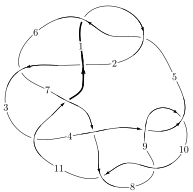
\includegraphics[width=112pt]{../../../GIT/diagram.site/Diagrams/png/326_11a_77.png}\\
\ \ \ A knot diagram\footnotemark}&
\allowdisplaybreaks
\textbf{Linearized knot diagam} \\
\cline{2-2}
 &
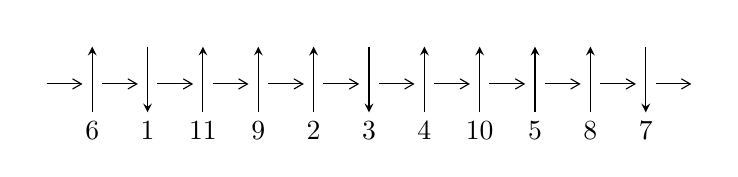
\begin{tikzpicture}[x=20pt, y=17pt]
	% nodes
	\node (C0) at (0, 0) {};
	\node (C1) at (1, 0) {};
	\node (C1U) at (1, +1) {};
	\node (C1D) at (1, -1) {6};

	\node (C2) at (2, 0) {};
	\node (C2U) at (2, +1) {};
	\node (C2D) at (2, -1) {1};

	\node (C3) at (3, 0) {};
	\node (C3U) at (3, +1) {};
	\node (C3D) at (3, -1) {11};

	\node (C4) at (4, 0) {};
	\node (C4U) at (4, +1) {};
	\node (C4D) at (4, -1) {9};

	\node (C5) at (5, 0) {};
	\node (C5U) at (5, +1) {};
	\node (C5D) at (5, -1) {2};

	\node (C6) at (6, 0) {};
	\node (C6U) at (6, +1) {};
	\node (C6D) at (6, -1) {3};

	\node (C7) at (7, 0) {};
	\node (C7U) at (7, +1) {};
	\node (C7D) at (7, -1) {4};

	\node (C8) at (8, 0) {};
	\node (C8U) at (8, +1) {};
	\node (C8D) at (8, -1) {10};

	\node (C9) at (9, 0) {};
	\node (C9U) at (9, +1) {};
	\node (C9D) at (9, -1) {5};

	\node (C10) at (10, 0) {};
	\node (C10U) at (10, +1) {};
	\node (C10D) at (10, -1) {8};

	\node (C11) at (11, 0) {};
	\node (C11U) at (11, +1) {};
	\node (C11D) at (11, -1) {7};
	\node (C12) at (12, 0) {};

	% arrows
	\draw[->,>={angle 60}]
	(C0) edge (C1) (C1) edge (C2) (C2) edge (C3) (C3) edge (C4) (C4) edge (C5) (C5) edge (C6) (C6) edge (C7) (C7) edge (C8) (C8) edge (C9) (C9) edge (C10) (C10) edge (C11) (C11) edge (C12) ;	\draw[->,>=stealth]
	(C1D) edge (C1U) (C2U) edge (C2D) (C3D) edge (C3U) (C4D) edge (C4U) (C5D) edge (C5U) (C6U) edge (C6D) (C7D) edge (C7U) (C8D) edge (C8U) (C9D) edge (C9U) (C10D) edge (C10U) (C11U) edge (C11D) ;
	\end{tikzpicture} \\
\hhline{~~} \\& 
\textbf{Solving Sequence} \\ \cline{2-2} 
 &
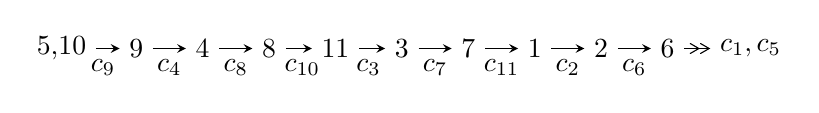
\begin{tikzpicture}[x=24pt, y=7pt]
	% node
	\node (A0) at (-1/8, 0) {5,10};
	\node (A1) at (1, 0) {9};
	\node (A2) at (2, 0) {4};
	\node (A3) at (3, 0) {8};
	\node (A4) at (4, 0) {11};
	\node (A5) at (5, 0) {3};
	\node (A6) at (6, 0) {7};
	\node (A7) at (7, 0) {1};
	\node (A8) at (8, 0) {2};
	\node (A9) at (9, 0) {6};
	\node (C1) at (1/2, -1) {$c_{9}$};
	\node (C2) at (3/2, -1) {$c_{4}$};
	\node (C3) at (5/2, -1) {$c_{8}$};
	\node (C4) at (7/2, -1) {$c_{10}$};
	\node (C5) at (9/2, -1) {$c_{3}$};
	\node (C6) at (11/2, -1) {$c_{7}$};
	\node (C7) at (13/2, -1) {$c_{11}$};
	\node (C8) at (15/2, -1) {$c_{2}$};
	\node (C9) at (17/2, -1) {$c_{6}$};
	\node (A10) at (41/4, 0) {$c_{1},c_{5}$};

	% edge
	\draw[->,>=stealth]	
	(A0) edge (A1) (A1) edge (A2) (A2) edge (A3) (A3) edge (A4) (A4) edge (A5) (A5) edge (A6) (A6) edge (A7) (A7) edge (A8) (A8) edge (A9) ;
	\draw[->>,>={angle 60}]	
	(A9) edge (A10);
\end{tikzpicture} \\ 

\end{tabular} \\

\footnotetext{
The image of knot diagram is generated by the software ``\textbf{Draw programme}" developed by Andrew Bartholomew(\url{http://www.layer8.co.uk/maths/draw/index.htm\#Running-draw}), where we modified some parts for our purpose(\url{https://github.com/CATsTAILs/LinksPainter}).
}\phantom \\ \newline 
\centering \textbf{Ideals for irreducible components\footnotemark of $X_{\text{par}}$} 
 
\begin{align*}
I^u_{1}&=\langle 
u^{65}+u^{64}+\cdots- u-1\rangle \\
\\
\end{align*}
\raggedright * 1 irreducible components of $\dim_{\mathbb{C}}=0$, with total 65 representations.\\
\footnotetext{All coefficients of polynomials are rational numbers. But the coefficients are sometimes approximated in decimal forms when there is not enough margin.}
\newpage
\renewcommand{\arraystretch}{1}
\centering \section*{I. $I^u_{1}= \langle u^{65}+u^{64}+\cdots- u-1 \rangle$}
\flushleft \textbf{(i) Arc colorings}\\
\begin{tabular}{m{7pt} m{180pt} m{7pt} m{180pt} }
\flushright $a_{5}=$&$\begin{pmatrix}0\\u\end{pmatrix}$ \\
\flushright $a_{10}=$&$\begin{pmatrix}1\\0\end{pmatrix}$ \\
\flushright $a_{9}=$&$\begin{pmatrix}1\\u^2\end{pmatrix}$ \\
\flushright $a_{4}=$&$\begin{pmatrix}- u\\- u^3+u\end{pmatrix}$ \\
\flushright $a_{8}=$&$\begin{pmatrix}- u^2+1\\u^2\end{pmatrix}$ \\
\flushright $a_{11}=$&$\begin{pmatrix}u^4- u^2+1\\- u^4\end{pmatrix}$ \\
\flushright $a_{3}=$&$\begin{pmatrix}u^{11}-2 u^9+4 u^7-4 u^5+3 u^3-2 u\\- u^{11}+u^9-2 u^7+u^5- u^3+u\end{pmatrix}$ \\
\flushright $a_{7}=$&$\begin{pmatrix}- u^6+u^4-2 u^2+1\\- u^8+2 u^6-2 u^4+2 u^2\end{pmatrix}$ \\
\flushright $a_{1}=$&$\begin{pmatrix}u^{18}-3 u^{16}+8 u^{14}-13 u^{12}+17 u^{10}-17 u^8+12 u^6-6 u^4+u^2+1\\u^{20}-4 u^{18}+10 u^{16}-18 u^{14}+23 u^{12}-24 u^{10}+18 u^8-10 u^6+3 u^4\end{pmatrix}$ \\
\flushright $a_{2}=$&$\begin{pmatrix}- u^{49}+8 u^{47}+\cdots+4 u^3- u\\- u^{51}+9 u^{49}+\cdots- u^3+u\end{pmatrix}$ \\
\flushright $a_{6}=$&$\begin{pmatrix}- u^{30}+5 u^{28}+\cdots-12 u^6+1\\u^{30}-4 u^{28}+\cdots-2 u^4+u^2\end{pmatrix}$\\ \flushright $a_{6}=$&$\begin{pmatrix}- u^{30}+5 u^{28}+\cdots-12 u^6+1\\u^{30}-4 u^{28}+\cdots-2 u^4+u^2\end{pmatrix}$\\&\end{tabular}
\flushleft \textbf{(ii) Obstruction class $= -1$}\\~\\
\flushleft \textbf{(iii) Cusp Shapes $= 4 u^{63}-40 u^{61}+\cdots+4 u+2$}\\~\\
\newpage\renewcommand{\arraystretch}{1}
\flushleft \textbf{(iv) u-Polynomials at the component}\newline \\
\begin{tabular}{m{50pt}|m{274pt}}
Crossings & \hspace{64pt}u-Polynomials at each crossing \\
\hline $$\begin{aligned}c_{1},c_{5}\end{aligned}$$&$\begin{aligned}
&u^{65}- u^{64}+\cdots+3 u-1
\end{aligned}$\\
\hline $$\begin{aligned}c_{2}\end{aligned}$$&$\begin{aligned}
&u^{65}+31 u^{64}+\cdots+u-1
\end{aligned}$\\
\hline $$\begin{aligned}c_{3}\end{aligned}$$&$\begin{aligned}
&u^{65}+7 u^{64}+\cdots+1657 u+101
\end{aligned}$\\
\hline $$\begin{aligned}c_{4},c_{9}\end{aligned}$$&$\begin{aligned}
&u^{65}+u^{64}+\cdots- u-1
\end{aligned}$\\
\hline $$\begin{aligned}c_{6}\end{aligned}$$&$\begin{aligned}
&u^{65}+u^{64}+\cdots-191 u-37
\end{aligned}$\\
\hline $$\begin{aligned}c_{7}\end{aligned}$$&$\begin{aligned}
&u^{65}- u^{64}+\cdots-7 u-1
\end{aligned}$\\
\hline $$\begin{aligned}c_{8},c_{10}\end{aligned}$$&$\begin{aligned}
&u^{65}-21 u^{64}+\cdots+u-1
\end{aligned}$\\
\hline $$\begin{aligned}c_{11}\end{aligned}$$&$\begin{aligned}
&u^{65}-5 u^{64}+\cdots+163 u-21
\end{aligned}$\\
\hline
\end{tabular}\\~\\
\newpage\renewcommand{\arraystretch}{1}
\flushleft \textbf{(v) Riley Polynomials at the component}\newline \\
\begin{tabular}{m{50pt}|m{274pt}}
Crossings & \hspace{64pt}Riley Polynomials at each crossing \\
\hline $$\begin{aligned}c_{1},c_{5}\end{aligned}$$&$\begin{aligned}
&y^{65}+31 y^{64}+\cdots+y-1
\end{aligned}$\\
\hline $$\begin{aligned}c_{2}\end{aligned}$$&$\begin{aligned}
&y^{65}+7 y^{64}+\cdots+9 y-1
\end{aligned}$\\
\hline $$\begin{aligned}c_{3}\end{aligned}$$&$\begin{aligned}
&y^{65}+19 y^{64}+\cdots+722417 y-10201
\end{aligned}$\\
\hline $$\begin{aligned}c_{4},c_{9}\end{aligned}$$&$\begin{aligned}
&y^{65}-21 y^{64}+\cdots+y-1
\end{aligned}$\\
\hline $$\begin{aligned}c_{6}\end{aligned}$$&$\begin{aligned}
&y^{65}-17 y^{64}+\cdots+2293 y-1369
\end{aligned}$\\
\hline $$\begin{aligned}c_{7}\end{aligned}$$&$\begin{aligned}
&y^{65}- y^{64}+\cdots+33 y-1
\end{aligned}$\\
\hline $$\begin{aligned}c_{8},c_{10}\end{aligned}$$&$\begin{aligned}
&y^{65}+47 y^{64}+\cdots-7 y-1
\end{aligned}$\\
\hline $$\begin{aligned}c_{11}\end{aligned}$$&$\begin{aligned}
&y^{65}+11 y^{64}+\cdots-30047 y-441
\end{aligned}$\\
\hline
\end{tabular}\\~\\
\newpage\flushleft \textbf{(vi) Complex Volumes and Cusp Shapes}
$$\begin{array}{c|c|c}  
\text{Solutions to }I^u_{1}& \I (\text{vol} + \sqrt{-1}CS) & \text{Cusp shape}\\
 \hline 
\begin{aligned}
u &= -0.689365 + 0.726697 I\end{aligned}
 & -1.58337 - 2.03293 I & \phantom{-}3.89738 + 3.26899 I \\ \hline\begin{aligned}
u &= -0.689365 - 0.726697 I\end{aligned}
 & -1.58337 + 2.03293 I & \phantom{-}3.89738 - 3.26899 I \\ \hline\begin{aligned}
u &= \phantom{-}1.005880 + 0.157008 I\end{aligned}
 & -0.41947 + 2.11288 I & \phantom{-}4.80416 - 3.07590 I \\ \hline\begin{aligned}
u &= \phantom{-}1.005880 - 0.157008 I\end{aligned}
 & -0.41947 - 2.11288 I & \phantom{-}4.80416 + 3.07590 I \\ \hline\begin{aligned}
u &= -0.911421 + 0.476290 I\end{aligned}
 & -0.02873 + 3.68623 I & \phantom{-}6.08412 - 2.12264 I \\ \hline\begin{aligned}
u &= -0.911421 - 0.476290 I\end{aligned}
 & -0.02873 - 3.68623 I & \phantom{-}6.08412 + 2.12264 I \\ \hline\begin{aligned}
u &= \phantom{-}0.687792 + 0.769063 I\end{aligned}
 & -0.78159 - 2.53862 I & \phantom{-}5.40480 + 3.10900 I \\ \hline\begin{aligned}
u &= \phantom{-}0.687792 - 0.769063 I\end{aligned}
 & -0.78159 + 2.53862 I & \phantom{-}5.40480 - 3.10900 I \\ \hline\begin{aligned}
u &= \phantom{-}1.030140 + 0.058702 I\end{aligned}
 & \phantom{-}3.90580 - 2.15177 I & \phantom{-}11.37394 + 2.20893 I \\ \hline\begin{aligned}
u &= \phantom{-}1.030140 - 0.058702 I\end{aligned}
 & \phantom{-}3.90580 + 2.15177 I & \phantom{-}11.37394 - 2.20893 I \\ \hline\begin{aligned}
u &= -1.029380 + 0.089417 I\end{aligned}
 & \phantom{-}5.09135 - 2.55649 I & \phantom{-}13.39578 + 4.21201 I \\ \hline\begin{aligned}
u &= -1.029380 - 0.089417 I\end{aligned}
 & \phantom{-}5.09135 + 2.55649 I & \phantom{-}13.39578 - 4.21201 I \\ \hline\begin{aligned}
u &= -1.037970 + 0.135001 I\end{aligned}
 & \phantom{-}4.01245 - 4.61295 I & \phantom{-}11.51833 + 4.52005 I \\ \hline\begin{aligned}
u &= -1.037970 - 0.135001 I\end{aligned}
 & \phantom{-}4.01245 + 4.61295 I & \phantom{-}11.51833 - 4.52005 I \\ \hline\begin{aligned}
u &= \phantom{-}0.908964 + 0.523673 I\end{aligned}
 & \phantom{-}1.93533 + 1.09584 I & \phantom{-}9.59662 - 2.36982 I \\ \hline\begin{aligned}
u &= \phantom{-}0.908964 - 0.523673 I\end{aligned}
 & \phantom{-}1.93533 - 1.09584 I & \phantom{-}9.59662 + 2.36982 I \\ \hline\begin{aligned}
u &= \phantom{-}1.047290 + 0.147978 I\end{aligned}
 & \phantom{-}1.79362 + 9.57441 I & \phantom{-}8.04394 - 8.42502 I \\ \hline\begin{aligned}
u &= \phantom{-}1.047290 - 0.147978 I\end{aligned}
 & \phantom{-}1.79362 - 9.57441 I & \phantom{-}8.04394 + 8.42502 I \\ \hline\begin{aligned}
u &= \phantom{-}0.694570 + 0.806772 I\end{aligned}
 & -2.33998 - 4.47857 I & \phantom{-}3.88200 + 0. I\phantom{ +0.000000I} \\ \hline\begin{aligned}
u &= \phantom{-}0.694570 - 0.806772 I\end{aligned}
 & -2.33998 + 4.47857 I & \phantom{-}3.88200 + 0. I\phantom{ +0.000000I} \\ \hline\begin{aligned}
u &= -0.693732 + 0.817224 I\end{aligned}
 & -4.71040 + 9.46363 I & \phantom{-0.000000 } 0. - 5.96163 I \\ \hline\begin{aligned}
u &= -0.693732 - 0.817224 I\end{aligned}
 & -4.71040 - 9.46363 I & \phantom{-0.000000 -}0. + 5.96163 I \\ \hline\begin{aligned}
u &= -0.855805 + 0.645921 I\end{aligned}
 & -2.22679 - 2.52501 I & \phantom{-0.000000 } 0 \\ \hline\begin{aligned}
u &= -0.855805 - 0.645921 I\end{aligned}
 & -2.22679 + 2.52501 I & \phantom{-0.000000 } 0 \\ \hline\begin{aligned}
u &= -0.714699 + 0.808408 I\end{aligned}
 & -6.81733 + 1.64607 I & \phantom{-0.000000 } 0 \\ \hline\begin{aligned}
u &= -0.714699 - 0.808408 I\end{aligned}
 & -6.81733 - 1.64607 I & \phantom{-0.000000 } 0 \\ \hline\begin{aligned}
u &= -0.786697 + 0.772614 I\end{aligned}
 & -3.96704 - 1.98381 I & \phantom{-0.000000 } 0 \\ \hline\begin{aligned}
u &= -0.786697 - 0.772614 I\end{aligned}
 & -3.96704 + 1.98381 I & \phantom{-0.000000 } 0 \\ \hline\begin{aligned}
u &= \phantom{-}0.770398 + 0.794763 I\end{aligned}
 & -7.77271 - 1.28375 I & \phantom{-0.000000 } 0 \\ \hline\begin{aligned}
u &= \phantom{-}0.770398 - 0.794763 I\end{aligned}
 & -7.77271 + 1.28375 I & \phantom{-0.000000 } 0\\
 \hline 
 \end{array}$$\newpage$$\begin{array}{c|c|c}  
\text{Solutions to }I^u_{1}& \I (\text{vol} + \sqrt{-1}CS) & \text{Cusp shape}\\
 \hline 
\begin{aligned}
u &= \phantom{-}0.946620 + 0.582707 I\end{aligned}
 & \phantom{-}2.30161 + 3.09152 I & \phantom{-0.000000 } 0 \\ \hline\begin{aligned}
u &= \phantom{-}0.946620 - 0.582707 I\end{aligned}
 & \phantom{-}2.30161 - 3.09152 I & \phantom{-0.000000 } 0 \\ \hline\begin{aligned}
u &= -0.843904 + 0.254405 I\end{aligned}
 & -1.51926 - 2.99365 I & \phantom{-}3.32010 + 5.42677 I \\ \hline\begin{aligned}
u &= -0.843904 - 0.254405 I\end{aligned}
 & -1.51926 + 2.99365 I & \phantom{-}3.32010 - 5.42677 I \\ \hline\begin{aligned}
u &= \phantom{-}0.800302 + 0.787738 I\end{aligned}
 & -6.57059 + 6.52849 I & \phantom{-0.000000 } 0 \\ \hline\begin{aligned}
u &= \phantom{-}0.800302 - 0.787738 I\end{aligned}
 & -6.57059 - 6.52849 I & \phantom{-0.000000 } 0 \\ \hline\begin{aligned}
u &= -0.966069 + 0.601492 I\end{aligned}
 & \phantom{-}0.74043 - 7.86664 I & \phantom{-0.000000 } 0 \\ \hline\begin{aligned}
u &= -0.966069 - 0.601492 I\end{aligned}
 & \phantom{-}0.74043 + 7.86664 I & \phantom{-0.000000 } 0 \\ \hline\begin{aligned}
u &= -0.944152 + 0.730238 I\end{aligned}
 & -3.48204 - 3.70053 I & \phantom{-0.000000 } 0 \\ \hline\begin{aligned}
u &= -0.944152 - 0.730238 I\end{aligned}
 & -3.48204 + 3.70053 I & \phantom{-0.000000 } 0 \\ \hline\begin{aligned}
u &= \phantom{-}0.937853 + 0.746992 I\end{aligned}
 & -6.14634 - 0.74794 I & \phantom{-0.000000 } 0 \\ \hline\begin{aligned}
u &= \phantom{-}0.937853 - 0.746992 I\end{aligned}
 & -6.14634 + 0.74794 I & \phantom{-0.000000 } 0 \\ \hline\begin{aligned}
u &= \phantom{-}0.800973\phantom{ +0.000000I}\end{aligned}
 & \phantom{-}1.17985\phantom{ +0.000000I} & \phantom{-}8.77650\phantom{ +0.000000I} \\ \hline\begin{aligned}
u &= -0.990290 + 0.689258 I\end{aligned}
 & -0.68502 - 3.40527 I & \phantom{-0.000000 } 0 \\ \hline\begin{aligned}
u &= -0.990290 - 0.689258 I\end{aligned}
 & -0.68502 + 3.40527 I & \phantom{-0.000000 } 0 \\ \hline\begin{aligned}
u &= \phantom{-}0.962070 + 0.741300 I\end{aligned}
 & -7.18458 + 7.06765 I & \phantom{-0.000000 } 0 \\ \hline\begin{aligned}
u &= \phantom{-}0.962070 - 0.741300 I\end{aligned}
 & -7.18458 - 7.06765 I & \phantom{-0.000000 } 0 \\ \hline\begin{aligned}
u &= \phantom{-}0.999686 + 0.703361 I\end{aligned}
 & \phantom{-}0.15648 + 8.12741 I & \phantom{-0.000000 } 0 \\ \hline\begin{aligned}
u &= \phantom{-}0.999686 - 0.703361 I\end{aligned}
 & \phantom{-}0.15648 - 8.12741 I & \phantom{-0.000000 } 0 \\ \hline\begin{aligned}
u &= -0.999377 + 0.728906 I\end{aligned}
 & -5.94902 - 7.42747 I & \phantom{-0.000000 } 0 \\ \hline\begin{aligned}
u &= -0.999377 - 0.728906 I\end{aligned}
 & -5.94902 + 7.42747 I & \phantom{-0.000000 } 0 \\ \hline\begin{aligned}
u &= \phantom{-}1.008600 + 0.721373 I\end{aligned}
 & -1.38595 + 10.22920 I & \phantom{-0.000000 } 0 \\ \hline\begin{aligned}
u &= \phantom{-}1.008600 - 0.721373 I\end{aligned}
 & -1.38595 - 10.22920 I & \phantom{-0.000000 } 0 \\ \hline\begin{aligned}
u &= -1.012630 + 0.725752 I\end{aligned}
 & -3.7395 - 15.2573 I & \phantom{-0.000000 } 0 \\ \hline\begin{aligned}
u &= -1.012630 - 0.725752 I\end{aligned}
 & -3.7395 + 15.2573 I & \phantom{-0.000000 } 0 \\ \hline\begin{aligned}
u &= -0.448985 + 0.508256 I\end{aligned}
 & -0.40000 + 3.37253 I & \phantom{-}3.73657 - 2.56528 I \\ \hline\begin{aligned}
u &= -0.448985 - 0.508256 I\end{aligned}
 & -0.40000 - 3.37253 I & \phantom{-}3.73657 + 2.56528 I \\ \hline\begin{aligned}
u &= -0.163452 + 0.613583 I\end{aligned}
 & -2.07374 - 7.24801 I & \phantom{-}0.44286 + 6.94914 I \\ \hline\begin{aligned}
u &= -0.163452 - 0.613583 I\end{aligned}
 & -2.07374 + 7.24801 I & \phantom{-}0.44286 - 6.94914 I \\ \hline\begin{aligned}
u &= \phantom{-}0.173474 + 0.573585 I\end{aligned}
 & \phantom{-}0.19197 + 2.46276 I & \phantom{-}3.81248 - 3.42438 I\\
 \hline 
 \end{array}$$\newpage$$\begin{array}{c|c|c}  
\text{Solutions to }I^u_{1}& \I (\text{vol} + \sqrt{-1}CS) & \text{Cusp shape}\\
 \hline 
\begin{aligned}
u &= \phantom{-}0.173474 - 0.573585 I\end{aligned}
 & \phantom{-}0.19197 - 2.46276 I & \phantom{-}3.81248 + 3.42438 I \\ \hline\begin{aligned}
u &= -0.088496 + 0.577660 I\end{aligned}
 & -3.86299 + 0.19977 I & -3.23482 + 0.27466 I \\ \hline\begin{aligned}
u &= -0.088496 - 0.577660 I\end{aligned}
 & -3.86299 - 0.19977 I & -3.23482 - 0.27466 I \\ \hline\begin{aligned}
u &= \phantom{-}0.302292 + 0.470945 I\end{aligned}
 & \phantom{-}1.11205 + 0.99447 I & \phantom{-}6.38117 - 3.96144 I \\ \hline\begin{aligned}
u &= \phantom{-}0.302292 - 0.470945 I\end{aligned}
 & \phantom{-}1.11205 - 0.99447 I & \phantom{-}6.38117 + 3.96144 I\\
 \hline 
 \end{array}$$\newpage
\newpage\renewcommand{\arraystretch}{1}
\centering \section*{ II. u-Polynomials}
\begin{tabular}{m{50pt}|m{274pt}}
Crossings & \hspace{64pt}u-Polynomials at each crossing \\
\hline $$\begin{aligned}c_{1},c_{5}\end{aligned}$$&$\begin{aligned}
&u^{65}- u^{64}+\cdots+3 u-1
\end{aligned}$\\
\hline $$\begin{aligned}c_{2}\end{aligned}$$&$\begin{aligned}
&u^{65}+31 u^{64}+\cdots+u-1
\end{aligned}$\\
\hline $$\begin{aligned}c_{3}\end{aligned}$$&$\begin{aligned}
&u^{65}+7 u^{64}+\cdots+1657 u+101
\end{aligned}$\\
\hline $$\begin{aligned}c_{4},c_{9}\end{aligned}$$&$\begin{aligned}
&u^{65}+u^{64}+\cdots- u-1
\end{aligned}$\\
\hline $$\begin{aligned}c_{6}\end{aligned}$$&$\begin{aligned}
&u^{65}+u^{64}+\cdots-191 u-37
\end{aligned}$\\
\hline $$\begin{aligned}c_{7}\end{aligned}$$&$\begin{aligned}
&u^{65}- u^{64}+\cdots-7 u-1
\end{aligned}$\\
\hline $$\begin{aligned}c_{8},c_{10}\end{aligned}$$&$\begin{aligned}
&u^{65}-21 u^{64}+\cdots+u-1
\end{aligned}$\\
\hline $$\begin{aligned}c_{11}\end{aligned}$$&$\begin{aligned}
&u^{65}-5 u^{64}+\cdots+163 u-21
\end{aligned}$\\
\hline
\end{tabular}\newpage\renewcommand{\arraystretch}{1}
\centering \section*{ III. Riley Polynomials}
\begin{tabular}{m{50pt}|m{274pt}}
Crossings & \hspace{64pt}Riley Polynomials at each crossing \\
\hline $$\begin{aligned}c_{1},c_{5}\end{aligned}$$&$\begin{aligned}
&y^{65}+31 y^{64}+\cdots+y-1
\end{aligned}$\\
\hline $$\begin{aligned}c_{2}\end{aligned}$$&$\begin{aligned}
&y^{65}+7 y^{64}+\cdots+9 y-1
\end{aligned}$\\
\hline $$\begin{aligned}c_{3}\end{aligned}$$&$\begin{aligned}
&y^{65}+19 y^{64}+\cdots+722417 y-10201
\end{aligned}$\\
\hline $$\begin{aligned}c_{4},c_{9}\end{aligned}$$&$\begin{aligned}
&y^{65}-21 y^{64}+\cdots+y-1
\end{aligned}$\\
\hline $$\begin{aligned}c_{6}\end{aligned}$$&$\begin{aligned}
&y^{65}-17 y^{64}+\cdots+2293 y-1369
\end{aligned}$\\
\hline $$\begin{aligned}c_{7}\end{aligned}$$&$\begin{aligned}
&y^{65}- y^{64}+\cdots+33 y-1
\end{aligned}$\\
\hline $$\begin{aligned}c_{8},c_{10}\end{aligned}$$&$\begin{aligned}
&y^{65}+47 y^{64}+\cdots-7 y-1
\end{aligned}$\\
\hline $$\begin{aligned}c_{11}\end{aligned}$$&$\begin{aligned}
&y^{65}+11 y^{64}+\cdots-30047 y-441
\end{aligned}$\\
\hline
\end{tabular}
\vskip 2pc
\end{document}